\documentclass[screen, acmtog]{acmart}

\AtBeginDocument{%
  \providecommand\BibTeX{{%
    Bib\TeX}}}

\acmDOI{XXXXXXX.XXXXXXX}

\begin{document}

\title{NEUROMORPHIC COMPUTING}

\author{Shiv Tikoo}
\affiliation{
  \institution{IIT Hyderabad}
  \city{}
  \country{India}
}

\author{Vishal Vijay Devadiga}
\affiliation{
  \institution{IIT Hyderabad}
  \city{}
  \country{India}
}

\keywords{Neuromorphic, Hardware, Architecture for Deep Learning, SNN, Memristor, Survey, Algorithms, Brain-Like Computing} 


\maketitle

\section{\textit{Abstract}}In the landscape of computational advancements, a new frontier has emerged, known as neuromorphic computing. This innovative approach, inspired by the intricate workings of the human brain, promises to transcend the boundaries of traditional Von Neumann architecture. This paper embarks on a journey through the recent developments in neuromorphic computing.

The advent of neuromorphic computing is a response to the escalating need for high-performance computing systems capable of managing complex tasks with superior efficiency. Conventional computing architectures are grappling with challenges related to speed, power consumption, and scalability. Neuromorphic computing, by emulating the neural structure of the brain, presents a potential resolution to these challenges.

At the heart of neuromorphic computing lie Spiking Neural Networks (SNNs). These networks deviate from traditional artificial neural networks by communicating through spikes, discrete events that occur at specific moments. This mode of communication mirrors the way neurons in the brain interact, leading to more efficient information processing. Another pivotal aspect of neuromorphic computing is Memristor technologies. Memristors, or memory resistors, are passive circuit elements that maintain a relationship between the time integrals of current and voltage across a device. Their unique properties make them ideal for implementing synaptic weights in neuromorphic systems.

As we look towards the future, neuromorphic computing is poised to play an increasingly significant role in the next generation of computing technologies. This abstract serves as a snapshot of the current state of neuromorphic computing and aims to pique interest in the detailed discussions that ensue in the rest of the paper. This paper is intended to be a valuable resource for those intrigued by the development and potential of neuromorphic computing.


\section{Introduction}

The journey of computing hardware development has been a testament to human ingenuity, transitioning from the room-sized mainframes of the past to the compact, high-performance devices that are now commonplace. Yet, as we continue to push the envelope of miniaturization, we are approaching the inherent limits of traditional computing architectures. The relentless pursuit of Moore’s Law, which foresaw a doubling of transistor density approximately every two years, is now confronting the challenges of diminishing returns as feature sizes near the atomic scale.

\begin{figure}
    \centering
    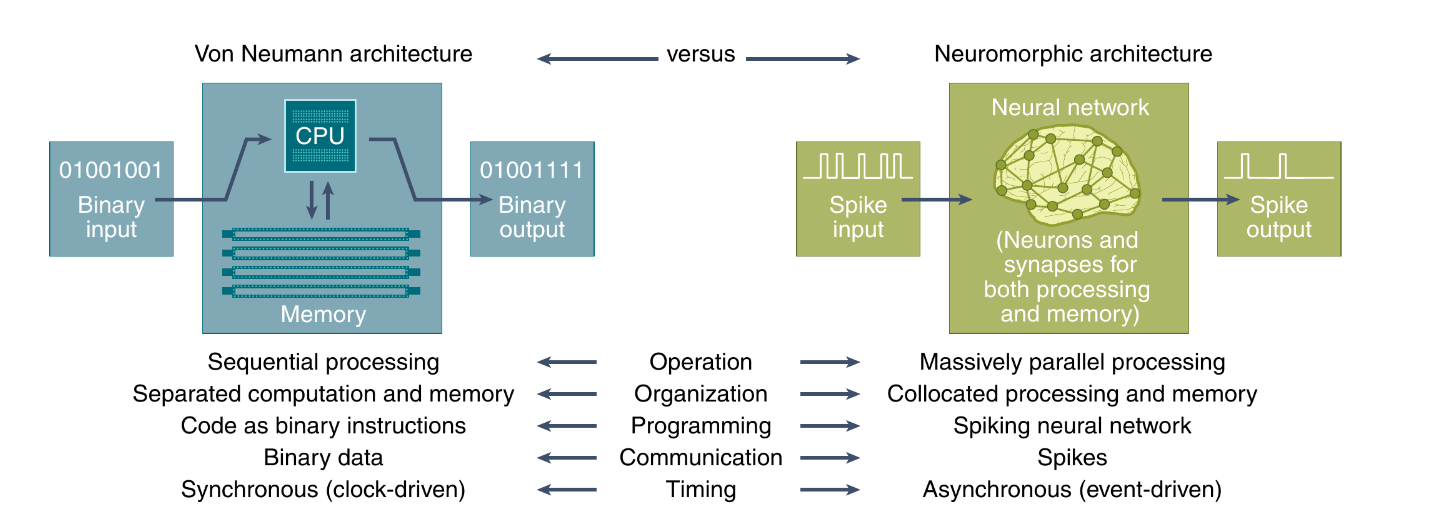
\includegraphics[width=1\linewidth]{comparevonneuro.png}
    \caption{Comparision of Von Neumann Architecture with Neuromorphic Architecture \cite{NCalgo}}
    \label{fig:comparevonneuro}
\end{figure}

\subsection{Need for Neuromorphic Computing} 

The evolution of computing hardware has been a cornerstone of technological progress over the past several decades. Reflecting on the fact that the first computer was the size of a room and had less processing power than a modern calculator, the strides made are truly extraordinary and have revolutionized the way we live and work. However, the current paradigm of computing is nearing its limits in terms of speed, power consumption, and scalability. Coupled with the exponential growth of data generation, there is a pressing need for a new computing paradigm that can keep pace with the demands of the modern world. Neuromorphic computing is anticipated to be this new paradigm and holds the potential to revolutionize our approach to computing.

The human brain, a highly complex organ, is capable of processing vast amounts of information in parallel. It is estimated that the human brain comprises around 100 billion neurons and 100 trillion synapses. The brain is also remarkably energy efficient, operating at a low frequency of around 100 Hz and consuming only about 20 watts of power. In stark contrast, modern supercomputers consume megawatts of power and operate at frequencies of several gigahertz. The human brain’s ability to learn and adapt to new situations remains a challenge for traditional computers. Neuromorphic computing, inspired by the human brain, seeks to emulate the way the brain processes information and is expected to be more efficient than traditional computing.


\subsection{Background}

The concept of Neuromorphic computing was first introduced by Carver Mead in the 1980s. The idea is based on using Very-Large-Scale Integration (VLSI) circuits with analog components to simulate the behavior of neurons in the brain. This stands in stark contrast to traditional computing, which is based on digital logic gates. Such systems use transistors to simulate the behavior of neurons and synapses and communicate with each other using impulses of electrical activity. This inspired the development of Spiking Neural Networks (SNNs) and Hybrid Neural Networks (HNNs).

SNNs are a type of artificial neural network that are inspired by the way the brain processes information. They are made up of spiking neurons that communicate with each other using spikes of electrical activity. These neurons do not have a fixed firing rate and only fire when their membrane potential reaches a certain threshold. SNNs have several advantages and disadvantages compared to traditional artificial neural networks. One of the main advantages is that they are more energy efficient and can achieve higher levels of performance. However, they are also more difficult to train and require more complex hardware. HNNs were first developed to retain the respective advantages of both SNNs and ANNs. In computer vision, for example, researchers use ANNs to extract features from images and then use SNNs to process these features.

There is a tremedous amount of research being done in developing new types of materials and devices that can be used to implement neuromorphic systems. Silicon-based devices have been the mainstay of the semiconductor industry for several decades, but they are reaching their physical limits in terms of size and power consumption. New materials such as phase change memory, memristors, ferroelectric materials and channel-doped biomembrances are being developed. Each of these materials has its own advantages and disadvantages, and researchers are working on developing new devices that can take full advantage of their capabilities.

Over the years, researchers have developed several different types of neuromorphic hardware. Some of the most notable include Neurogrid by Stanford University, SpiNNaker by the University of Manchester, TrueNorth by IBM, and Loihi by Intel. All of these systems are based on the idea of using analog components to simulate the behavior of neurons and synapses. They are also highly parallel and can process vast amounts of information in real time. Loihi, for example, is capable of simulating the behavior of 130,000 neurons across its 128 neuromorphic cores and 3 x86 cores. Extended clusters of up to 768 Loihi Chips operate at 500 watts of power and can simulate the behavior of 100 million neurons.

Tianjic is another neuromorphic chip developed by Tsinghua University in China. Released in 2014, it offered a peak internal storage bandwidth of 610 GBps. It generated a lot of interest in the field of neuromorphic computing due to its high performance, energy efficiency, and software toolchain. The university also developed a robotic system that was controlled by Tianjic and was capable of performing tasks such as object recognition, navigation, and manipulation.
\section{Survey}

Neuromorphic computing is still in its infancy and there are many challenges that need to be overcome before it can be widely adopted. This paper will discuss some of the challenges, solutions and potential area of research in neuromorphic computing that include hardware design, architecture, algorithms, and applications. \\
Below are some of the key challenges in neuromorphic computing:

\begin{itemize}
    \item Hardware design: Neuromorphic hardware is still in the early stages of development and there are many challenges to be overcome in terms of design and fabrication. For example, memristors are a promising new technology that could be used to implement neuromorphic systems, but there are still many challenges to be overcome in terms of fabrication and integration with existing technologies.
    \item Architecture: Neuromorphic systems are highly parallel and require specialized architectures to take full advantage of their capabilities. There are still many challenges to be overcome in terms of designing efficient and scalable architectures for neuromorphic systems.
    \item Algorithms: Neuromorphic systems require specialized algorithms to take full advantage of their capabilities. There are still many challenges to be overcome in terms of developing algorithms that are efficient and scalable for neuromorphic systems.
    \item Applications: Neuromorphic systems have the potential to revolutionize many different fields, but there are still many challenges to be overcome in terms of developing applications that can take full advantage of their capabilities.
\end{itemize}

\subsection{Spiking Neural Networks}

Spiking Neural Networks (SNNs) are a type of artificial neural network that takes inspiration from the functioning of biological neural networks. Unlike traditional neural networks that transmit information as continuous values, SNNs transmit information as discrete spikes, mimicking the “fire-and-forget” manner of real neurons. This event-driven nature of SNNs opens up novel research directions and has the potential to achieve lower power consumption.

The relevance of SNNs to neuromorphic computing is profound. Neuromorphic computing, by design, seeks to mimic the human brain’s structure and function – and SNNs provide a computational model that aligns with this goal. By leveraging the discrete, spike-based communication of SNNs, neuromorphic computing can potentially achieve high computational efficiency, low power consumption, and robust performance, much like the human brain. The advent of SNNs in neuromorphic computing marks a significant shift in the computational paradigm. Traditional computing systems, with their clock-driven synchronous operations and energy-intensive processes, are reaching their physical limits. In contrast, neuromorphic computing systems with SNNs operate asynchronously, leading to potential advantages in speed, power efficiency, and real-time processing capabilities.

This shift towards SNN-based neuromorphic computing is not just a technological evolution; it’s a paradigm shift that could redefine what is possible in the realm of artificial intelligence and machine learning. As we delve deeper into the survey, we will explore how this paradigm is being realized in current research and applications.

In the following subsection, we delve into a curated selection of papers that exemplify the advancements and applications of SNNs in the field of neuromorphic computing. Through these papers, we aim to gain insights into the current state-of-the-art techniques, challenges, and future directions in this rapidly evolving domain, having gained an understanding of SNNs, let us now delve deeper into the field with the examination of a recent and pivotal paper titled \textit{Exploring Neuromorphic Computing Based on Spiking Neural Networks: Algorithms to Hardware}.


This work\cite{Spiking} takes a holistic approach, delving into the intricate interplay between algorithms and hardware architectures in the context of SNNs. At its core, the paper advocates for a paradigm shift in computational design, aiming to emulate the efficiency and adaptability of the human brain.

The cornerstone of this paper lies in the notion of multi-stack optimization, a concept that defies conventional compartmentalization. Here, optimization extends across devices, circuits, and algorithms, intertwining their functionalities in a harmonious symphony. This unified approach endeavors to emulate the brain's natural prowess in information processing, striving for unparalleled efficiency. A particularly intriguing aspect of the paper is its exploration of data representation in spike-trains. Drawing inspiration from neurobiology, the authors propose encoding data as sequences of discrete spikes, mirroring the asynchronous communication observed in biological neurons. This innovative approach holds promise for enhancing the efficiency and scalability of neuromorphic systems.

Moreover, the paper elucidates novel neuron models tailored to capture the nuanced temporal dynamics of biological neurons. By incorporating temporal processing capabilities, these models enable SNNs to more faithfully emulate the brain's intricate information processing mechanisms, unlocking new frontiers in cognitive computing. The authors also tackle the formidable challenge of designing learning algorithms optimized for event-driven dynamical systems. By embracing the inherently asynchronous nature of SNNs, these algorithms adapt dynamically to environmental stimuli, paving the way for robust and adaptive neuromorphic systems. Beyond technical innovations, the paper provides a thought-provoking exploration of the broader challenges and opportunities in neuromorphic computing. It underscores the pressing need for interdisciplinary collaboration and continued research across algorithmic development, hardware design, and system optimization to realize the full potential of SNN-based architectures. In essence, it offers a captivating glimpse into the future of computing. By seamlessly integrating insights from neuroscience, computer science, and engineering, the paper charts a course towards a new era of intelligent computing systems that rival the capabilities of the human brain.

Embarking on a journey from theory to reality, with the next paper we explored how SNNs team up with neuromorphic architectures\cite{SNNreview}. These neuromorphic architectures, meticulously crafted to mimic the intricate neural structures of the human brain, provide an ideal substrate for the integration of SNNs. Unlike their traditional counterparts, SNNs operate by transmitting discrete spikes of information, echoing the firing patterns observed in biological neurons. Within this intricate ecosystem, system software frameworks emerge as indispensable enablers, furnishing the requisite infrastructure for deploying machine learning applications on neuromorphic hardware. These frameworks serve as orchestrators, seamlessly facilitating the intricate interplay between algorithms and hardware components, thereby streamlining the design, training, and deployment of SNNs on neuromorphic architectures.

The paper under scrutiny embarks on a meticulous exploration of the multifaceted challenges inherent in integrating SNNs with neuromorphic architectures. Navigating through the intricate landscape of system software frameworks, the authors adeptly navigate issues related to performance optimization, energy efficiency, and reliability. Through a nuanced examination, they underscore the urgent imperative for robust frameworks capable of accommodating the ever-mounting complexity of machine learning applications on neuromorphic systems. At the core of their discourse lies the meticulous delineation of system software frameworks tailored to cater to both platform-based design and hardware-software co-design paradigms. By meticulously dissecting the diverse array of existing frameworks, the authors meticulously lay out a roadmap for future endeavors in system software technology for neuromorphic computing. They meticulously outline the contours of prospective investigations, beckoning towards innovative solutions that seamlessly integrate software sophistication with hardware prowess.

\begin{figure}
    \centering
    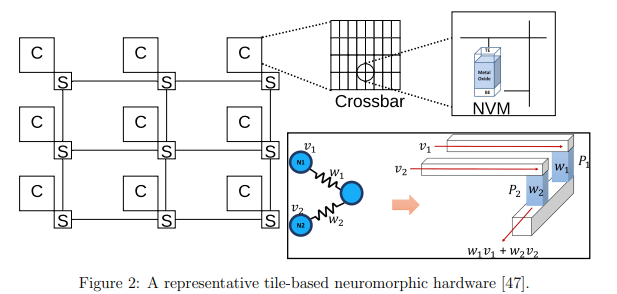
\includegraphics[width=1\linewidth]{Screenshot from 2024-04-28 20-11-45.png}
    \caption{A representative tile-based neuromorphic hardware \cite{SNNreview}}
    \label{fig:NC HW}
\end{figure}

In essence, this paper serves as a guiding beacon, illuminating the practical pathways towards realizing the symbiotic relationship between SNNs and neuromorphic architectures. It underscores the indispensable role of robust system software frameworks and charts a definitive course towards the future of system software technology in the realm of neuromorphic computing.

Neuromorphic systems, with their intricate integration of neurons and synapses, are susceptible to faults that can compromise system reliability. As the complexity of these systems grows, so does the vulnerability of their hardware implementations. The intricacies hidden within these accelerators can be exploited by attackers through various side-channel information, posing a significant security risk. However, the inherent spike-based computation in neuromorphic systems offers resilience against transient faults, as the impact of faulty spikes can often be mitigated. Yet, permanent and intermittent faults can still disrupt the functionality of modules within neuromorphic systems, leading to inaccuracies in results. Given these challenges, the development of robust fault-tolerant mechanisms becomes paramount for ensuring the practical implementation and reliability of neuromorphic systems. This area of research is actively pursued within the field of neuromorphic computing, aiming to address the growing concerns surrounding system reliability and security.

The final paper for this subsection is directly aimed at this pitfall and presents a significant advancement in the field of neuromorphic computing by introducing a groundbreaking scalable neuromorphic fault-tolerant context-dependent learning (FCL) hardware framework\cite{FaultTolerant}. This framework represents a significant advancement, offering resilience against faults while enabling effective learning in context-dependent tasks, even in the presence of hardware failures. Addressing the critical issue of fault-tolerance in neuromorphic systems, the authors provide insights into the development of a framework capable of maintaining robust learning capabilities despite potential hardware faults. This breakthrough not only mitigates the challenges associated with fault-tolerant on-chip learning but also opens up new possibilities for the design and implementation of resilient neuromorphic systems.

Furthermore, the paper delves into the broader landscape of neuromorphic computing, emphasizing the need for continued research in fault-tolerant learning mechanisms and hardware design paradigms. It advocates for the development of robust learning frameworks that can adeptly manage faults, ensuring the reliable operation of neuromorphic systems in real-world applications. It not only addresses present challenges but also sets the stage for future advancements, propelling the development of more dependable and efficient neuromorphic systems.

\subsection{Algorithms for Neuromorphic Systems \cite{NCalgo}}

Considering that neuromorphic architecture are highly parallelizable and inherently scalable, there is a need for specialized algorithms that can take full advantage of their capabilities. One of the key challenges in neuromorphic computing is developing algorithms that are efficient and scalable. Traditional algorithms that are used in artificial neural networks may not be well suited for neuromorphic systems. 

Below are some examples of specialized algorithms that have been developed for neuromorphic systems:

\begin{figure*}
    \centering
    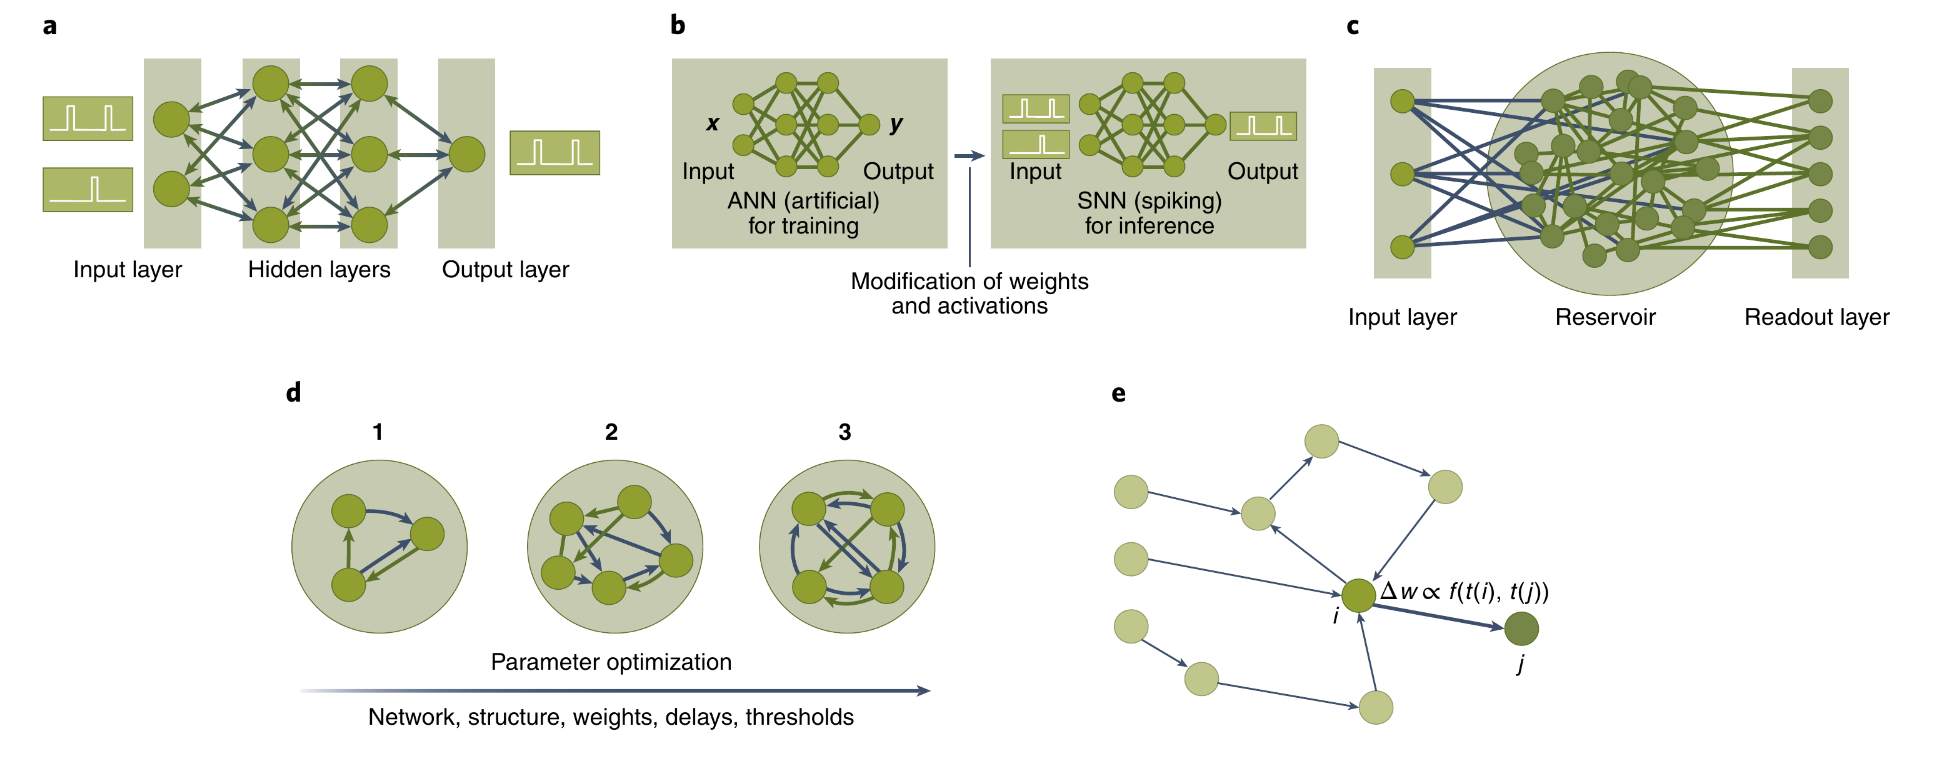
\includegraphics[width=1\linewidth]{algoNC.png}
    \caption{\cite{NCalgo} (a): Spike-based Quasi-backpropgation (b): Mapping ANNs to SNNs (c): Resevoir Computing (d): Evolution of SNNs over time (e): Time Parameter in spikes}
    \label{fig:AlgoNC}
\end{figure*}

\begin{itemize}
    \item Backpropagation, which is a popular algorithm for training artificial neural networks, may not be well suited for neuromorphic systems due to its high computational complexity and memory requirements. Also the fact that SNNs are inherently stochastic and non-deterministic, makes it difficult to train them using traditional backpropagation algorithms. \textit{Spike-based quasi-backpropagation} adapt the backpropagation algorithm to work with SNNs by using surrogate gradients and smoothed actiobation functions to compute the gradients while maintaining the spiking behavior of the neurons.
    \item Since ANNs have a long history of research, there are many algorithms and optimizations that have been developed for them. Performing a \textit{mapping} process from ANNs to SNNs is a challenging task, but inherently leads to better performance with respect to energy efficiency and speed. However this mapping process can lead to loss of accuracy due to the conversion of continuous values to spikes. 
    \item \textit{Resevoir Computing} is a popular algorithm used in neuromorphic systems that is based on the idea of using a large network of recurrently connected neurons to perform computations. The network does not involve any training of the SNN components. It uses sparse connectivity and random weights to cast inputs to a higher dimensiontality space. The output is then read out from the network using a linear classifier. Resevoir computing has been shown to be highly efficient and scalable and has been used in a wide range of applications.
    \item \textit{Evolutionary Approaches} is another popular algorithm used in neuromorphic systems that is based on the idea of using multiple generations of populations and selecting the best individuals to evolve the population. This approach can be used to optimize the parameters of the SNNs and is highly efficient and scalable as it does not require any differentiablity in activation functions nor rely on any particular network structure
\end{itemize}

Neuromorphic Computing can be used in a wide range of applications, including non-ML tasks such as signal processing, graph theory, and optimization. For example, during the pandemic in 2020, researchers used neuromorphic computing to develop a model that could predict the spread of COVID-19. 

However there are still many challenges to be overcome in terms of developing algorithms that are efficient and scalable for neuromorphic systems. There is not yet a ML algorithm that substantially outperforms traditional ML algorithms in terms of accuracy, speed, and energy efficiency. This leads to the argument that neuromorphic computing is useful for its low power computing abilities.

Another key challenge is the lack of a standard benchmark for evaluating neuromorphic algorithms. There are many different neuromorphic systems available, each with its own architecture and capabilities. This makes it difficult to compare the performance of different algorithms across different systems. There is a need for a standard benchmark that can be used to evaluate the performance of neuromorphic algorithms and systems.

\subsection{CerebelluMorphic\cite{CerebelluMorphic} and BiCoSS\cite{BiCoss}}

BiCoSS and CerebelluMorphic are two neuromorphic systems that have been developed in recent years. Considering both these papers were published in 2022 and by the same group, they share some common design principles.

\begin{figure}
    \centering
    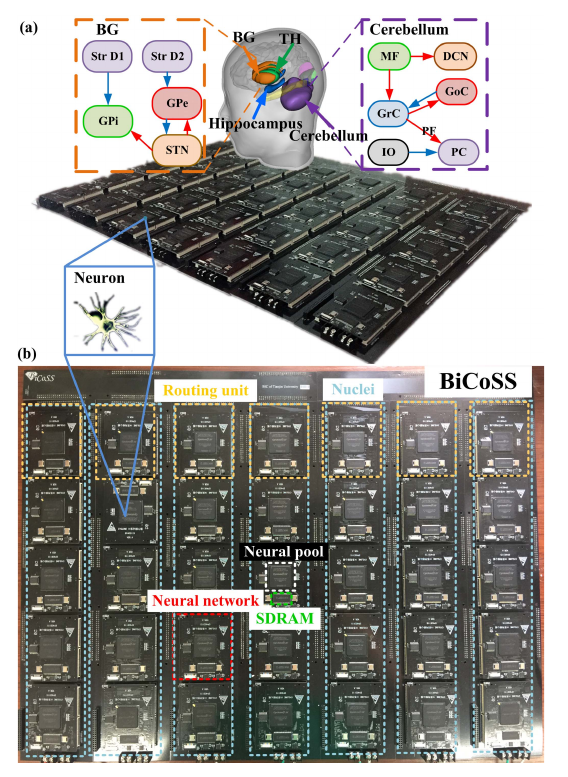
\includegraphics[width=0.8\linewidth]{bicoss.png}
    \caption{\cite{BiCoss} (a): Brain Cognitive Functions implemented in BiCoSS  \\ (b): BiCoSS System}
    \label{fig:bicoss}
\end{figure}

BiCoSS uses scalable hierachical heterogeneous multicore architecture with localized memory. By determining neuron models for multiple cognitive organs such as the cerebellum, hippocampus, and basal ganglia, and many more, BiCoSS can construct biological cognitive systems. It has 3 main design principles:

\begin{itemize}
    \item Independency Reconfigurable Population Process: Using FPGAs, the system can be reconfigured to perform different tasks of different complexity. This allows for the system to be used in a wide range of applications. 
    \item Stochastic Neural Heterogenity: BiCoSS presents an efficient alogrithm for optimizing temporal and spatial heterogenity in the neural network, meaning that the response of the neurons can be optimized with respect to the intensity of the input. This allows for the system to be more energy efficient and faster. It also allows for the system to be more robust to noise and other disturbances.
    \item Routing Scheme for Hybrid Neural information: Different synapses have different spiking activities, and synaptic dynamics. 1 bit calculations are realized by multiplexer. This allows for the system to be mimic the behavior of various cognitive organs.
\end{itemize}

CerebelluMorphic is a neuromorphic system that is inspired by the cerebellum, which is a part of the brain that is responsible for motor control and coordination. The cerebellum is highly efficient and is capable of processing vast amounts of information in real time. CerebelluMorphic is based on the idea of using a large network of spiking neurons to simulate the behavior of the cerebellum. 

A key challenge in neuromorphic computing is acheiving further brain complexity. The human brain is highly complex and is capable of processing vast amounts of information in parallel. These two architecture are just the beginning of realizing large-scale brain models and lay the groundwork for further research in the field of neuromorphic computing.

\subsection{Memristors\cite{MemristorProgress}}

Memristance is a property of an electronic component that is capable of changing its resistance in response to the amount of current that flows through it. Materials that exhibit memristance are called memristors. A memristor is a two-terminal electronic device whose resistance depends on the voltage applied to it and the length of time that voltage has been applied. This property allows memristors to retain information even when the power is turned off, making them ideal for memory storage. Memristors have been proposed as a possible solution to the challenges of neuromorphic computing as they can adjust their resistance based on the amount and timing of the voltage applied across them, mimicking the plasticity of biological synapses and enabling learning and adaptation considering that transistor technology, as it is currently implemented, is reaching its physical limits in terms of size and power consumption.

Memristors were first proposed by Leon Chua in 1971, but it wasn't until 2008 that the first practical memristor was developed by HP Labs. Since then, memristors have been the subject of intense research and development, with many companies and research institutions working on developing memristor-based devices.

Memristors have several advantages over traditional transistors.

\begin{itemize}
    \item \textbf{Non-volatile memory}: Memristors retain their state even when the power is turned off. This makes them ideal for use in memory devices.
    \item \textbf{Low power consumption}: Memristors consume less power than traditional transistors. This is because they do not require a constant flow of current to maintain their state.
    \item \textbf{High density}: Memristors can be packed more densely than traditional transistors. Memristors can also store multiple bits of data per cell, further increasing their density. Multiple sturctures have been proposed for memristors, such as the crossbar array, which allows for high density and parallel processing, or cubes of memristors, which allow for 3D integration.
\end{itemize}

However, memristors also have some disadvantages.

\begin{itemize}
    \item \textbf{Reliability issues}: Memristors can be prone to errors in conductance leading to data corruption. This can be a problem in applications that require high reliability. Thus, effective solutions to mitigate these errors are needed.
    \item \textbf{Fabrication challenges}: Memristors are still in the early stages of development and there are still many challenges to be overcome in terms of fabrication and integration with existing technologies.
\end{itemize}

\begin{figure}
    \centering
    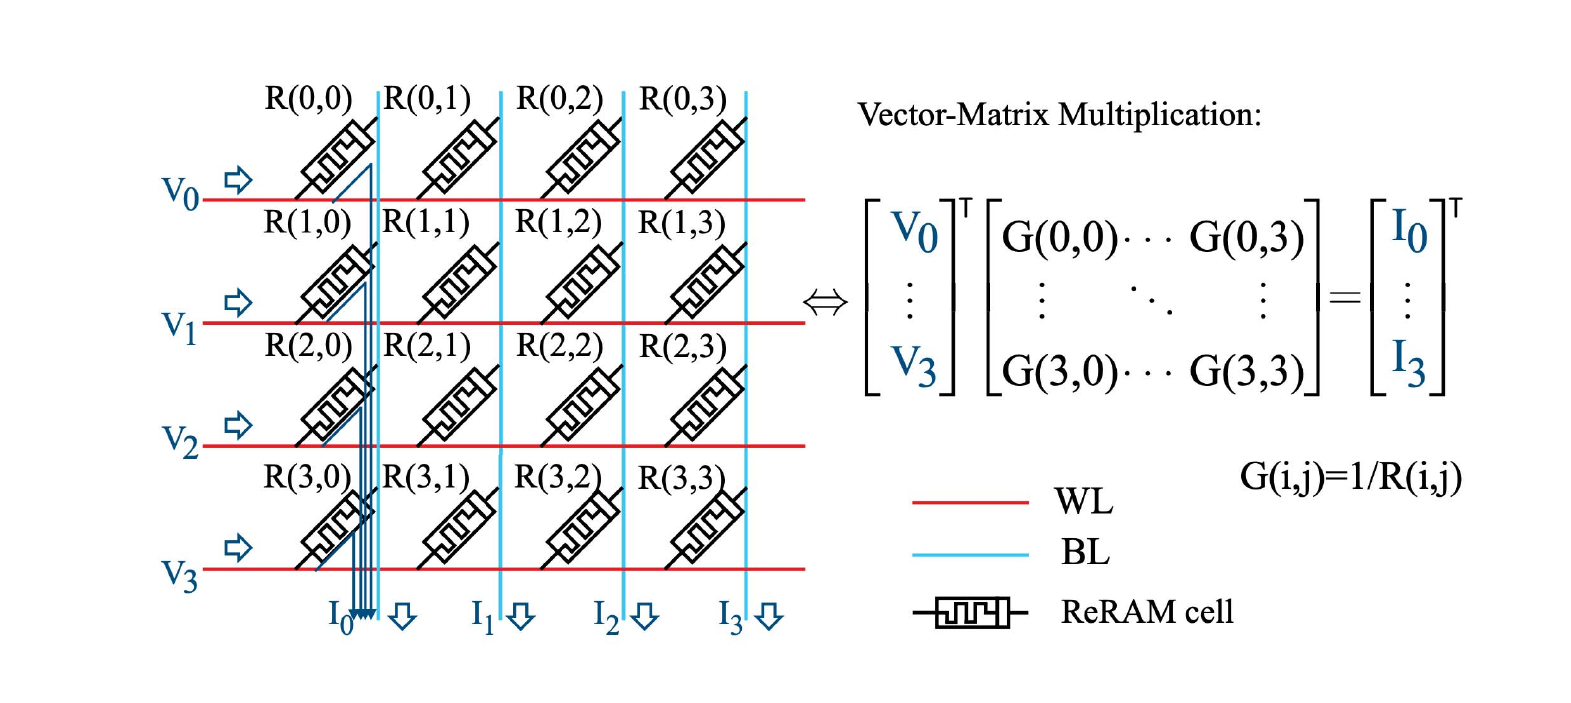
\includegraphics[width=1\linewidth]{memristor-crossbar.png}
    \caption{Memristor Crossbars - based Matrix Multiplication \cite{MemristorProgress}}
    \label{fig:mem-cross}
\end{figure}

Memristor Crossbars are of much relevance in the field of neural networks. Due to their structure, they can be used to implement vector matrix multiplication, which is a key operation in neural networks. Figure \ref{fig:mem-cross} shows a simple crossbar array with memristors. On applying a voltage to the input lines, the memristors change their resistance based on the voltage applied. The output lines then read the resistance of the memristors, which is proportional to the dot product of the input and weight vectors. This allows for parallel processing of multiple inputs and weights, making it ideal for neural networks.

Using memristors in neuromorphic computing instead of traditional transistors has several advantages. 

\begin{itemize}
    \item State retention: Memristors retain their state even when the power is turned off. This makes them ideal for use in memory devices.
    \item State representation: Conductance of a memristor can be used to represent the synaptic weight between two neurons. This allows for the implementation of synapses in neuromorphic systems.
    \item As mentioned earlier, memristors can be used to implement vector matrix multiplication, which is a key operation in neural networks. This allows for the implementation of neural networks in hardware, which can be much faster and more energy efficient than software implementations.
\end{itemize}

Thus, memristors have the potential to revolutionize the field of neuromorphic computing and enable the development of more efficient and powerful neuromorphic systems once the challenges of fabrication and reliability are overcome.

\section{Conclusion}

Neuromorphic computing is a promising new computing paradigm that has the potential to revolutionize the way we think about computing. By mimicking the way the brain processes information, neuromorphic systems are expected to be more efficient and powerful than traditional computing systems. 

\begin{figure}
    \centering
    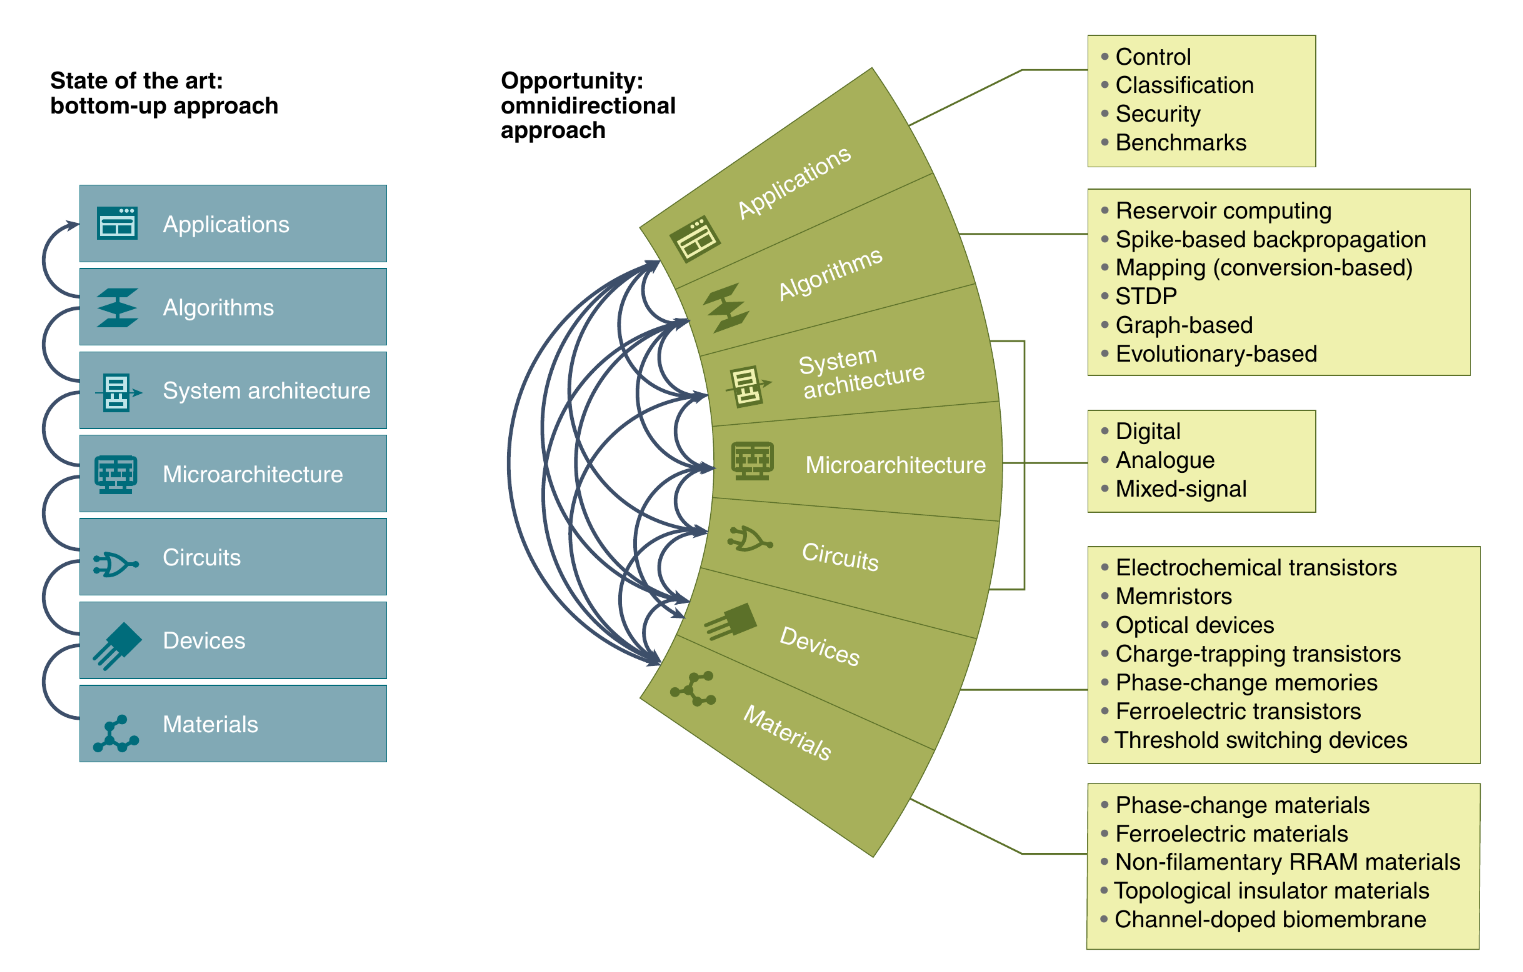
\includegraphics[width=1\linewidth]{oppurtunities.png}
    \caption{Opportunities in Neuromorphic Computing \cite{NCalgo}}
    \label{fig:opportunities}
\end{figure}

Over the years, researchers have developed several different types of neuromorphic hardware, architecture, and algorithms. Considering that the human brain is capable of processing vast amounts of information in parallel, neuromorphic systems are highly parallel and can process vast amounts of information in real time. Several large-scale neuromorphic systems have been developed and are available for research and development.

However, there are still many challenges that need to be overcome before neuromorphic computing can be widely adopted. Various functions of the brain are still not fully understood, and reverse engineering the brain is a complex and challenging task. 

There are also many challenges in software-hardware co-design. Currently most neuromorphic research is focused on individual aspects of neuromorphic systems, such as hardware design, architecture, algorithms, and applications. There is a need for more research that integrates these different aspects and develops holistic solutions that take full advantage of the capabilities of neuromorphic systems.

Integration of such systems is quite difficult because they encompass a wide range of technologies and disciplines. There is a need for more collaboration between researchers in different fields and more interdisciplinary research that can address the challenges of neuromorphic computing.

By addressing these challenges, researchers can help to unlock the full potential of neuromorphic computing and usher in a new era of computing.

\section{Acknowledgements}
We would like to thank:
\begin{itemize}
    \item Professor Rajesh Kedia
    \item Professor Shirshendu Das
\end{itemize}
for guiding us, and teaching the course "CS6490: Hardware Architecture for Deep Learning" at Indian Institute of Technology, Hyderabad

% \section{References}


% \begin{enumerate}

%     \item[] [1]: Paper\cite{Schuman2022}
%     \item[] [2]: "BiCoSS: Toward Large-Scale Cognition Brain With Multigranular Neuromorphic Architecture" - IEEE TRANSACTIONS ON NEURAL NETWORKS AND LEARNING SYSTEMS, VOL. 33, NO. 7, JULY 2022
%     \item[] [3]: "CerebelluMorphic: Large-Scale Neuromorphic Model and Architecture for Supervised Motor Learning" - IEEE TRANSACTIONS ON NEURAL NETWORKS AND LEARNING SYSTEMS, VOL. 33, NO. 9, SEPTEMBER 2022
%     \item[] [4]: "Research Progress on Memristor: From Synapses to Computing Systems" - IEEE TRANSACTIONS ON CIRCUITS AND SYSTEMS—I: REGULAR PAPERS, VOL. 69, NO. 5, MAY 2022 
%     \item[] [5]: "Opportunities for neuromorphic computing
% algorithms and applications" - Nature Computational Science 2, 10-19 (2022)\cite{5}
%     \item[] [6]: S. Yang, J. Wang, B. Deng, M. R. Azghadi and B. Linares-Barranco, "Neuromorphic Context-Dependent Learning Framework With Fault-Tolerant Spike Routing," in IEEE Transactions on Neural Networks and Learning Systems, vol. 33, no. 12, pp. 7126-7140, Dec. 2022, doi: 10.1109/TNNLS.2021.3084250.
% keywords: {Neuromorphics;Neurons;Fault tolerant systems;Brain modeling;Task analysis;Context modeling;Brain modeling;Neural networks;Brain inspired;context-dependent learning;fault tolerant;neuromorphic computing;spiking neural network (SNN)},


%     \item[] [7]:
%     \item[] [8]:

% \end{enumerate}

% \cite{BiCoss}
% \cite{CerebelluMorphic}
% \cite{FaultTolerant}
% \cite{MemristorProgress}
% \cite{NCalgo}
% \cite{SNNreview}
% \cite{Spiking}
% \cite{extra}


\bibliographystyle{plain}
\bibliography{sample-base}




\end{document}



% \section{Sectioning Commands}

% Your work should use standard \LaTeX\ sectioning commands:
% \verb|section|, \verb|subsection|, \verb|subsubsection|, and
% \verb|paragraph|. They should be numbered; do not remove the numbering
% from the commands.

% Simulating a sectioning command by setting the first word or words of
% a paragraph in boldface or italicized text is {\bfseries not allowed.}

% \section{Tables}

% The ``\verb|acmart|'' document class includes the ``\verb|booktabs|''
% package --- \url{https://ctan.org/pkg/booktabs} --- for preparing
% high-quality tables.

% Table captions are placed {\itshape above} the table.

% Because tables cannot be split across pages, the best placement for
% them is typically the top of the page nearest their initial cite.  To
% ensure this proper ``floating'' placement of tables, use the
% environment \textbf{table} to enclose the table's contents and the
% table caption.  The contents of the table itself must go in the
% \textbf{tabular} environment, to be aligned properly in rows and
% columns, with the desired horizontal and vertical rules.  Again,
% detailed instructions on \textbf{tabular} material are found in the
% \textit{\LaTeX\ User's Guide}.

% Immediately following this sentence is the point at which
% Table~\ref{tab:freq} is included in the input file; compare the
% placement of the table here with the table in the printed output of
% this document.

% \begin{table}
%   \caption{Frequency of Special Characters}
%   \label{tab:freq}
%   \begin{tabular}{ccl}
%     \toprule
%     Non-English or Math&Frequency&Comments\\
%     \midrule
%     \O & 1 in 1,000& For Swedish names\\
%     $\pi$ & 1 in 5& Common in math\\
%     \$ & 4 in 5 & Used in business\\
%     $\Psi^2_1$ & 1 in 40,000& Unexplained usage\\
%   \bottomrule
% \end{tabular}
% \end{table}

% To set a wider table, which takes up the whole width of the page's
% live area, use the environment \textbf{table*} to enclose the table's
% contents and the table caption.  As with a single-column table, this
% wide table will ``float'' to a location deemed more
% desirable. Immediately following this sentence is the point at which
% Table~\ref{tab:commands} is included in the input file; again, it is
% instructive to compare the placement of the table here with the table
% in the printed output of this document.

% \begin{table*}
%   \caption{Some Typical Commands}
%   \label{tab:commands}
%   \begin{tabular}{ccl}
%     \toprule
%     Command &A Number & Comments\\
%     \midrule
%     \texttt{{\char'134}author} & 100& Author \\
%     \texttt{{\char'134}table}& 300 & For tables\\
%     \texttt{{\char'134}table*}& 400& For wider tables\\
%     \bottomrule
%   \end{tabular}
% \end{table*}

% Always use midrule to separate table header rows from data rows, and
% use it only for this purpose. This enables assistive technologies to
% recognise table headers and support their users in navigating tables
% more easily.

% \section{Math Equations}
% You may want to display math equations in three distinct styles:
% inline, numbered or non-numbered display.  Each of the three are
% discussed in the next sections.

% \subsection{Inline (In-text) Equations}
% A formula that appears in the running text is called an inline or
% in-text formula.  It is produced by the \textbf{math} environment,
% which can be invoked with the usual
% \texttt{{\char'134}begin\,\ldots{\char'134}end} construction or with
% the short form \texttt{\$\,\ldots\$}. You can use any of the symbols
% and structures, from $\alpha$ to $\omega$, available in
% \LaTeX~\cite{Lamport:LaTeX}; this section will simply show a few
% examples of in-text equations in context. Notice how this equation:
% \begin{math}
%   \lim_{n\rightarrow \infty}x=0
% \end{math},
% set here in in-line math style, looks slightly different when
% set in display style.  (See next section).

% \subsection{Display Equations}
% A numbered display equation---one set off by vertical space from the
% text and centered horizontally---is produced by the \textbf{equation}
% environment. An unnumbered display equation is produced by the
% \textbf{displaymath} environment.

% Again, in either environment, you can use any of the symbols and
% structures available in \LaTeX\@; this section will just give a couple
% of examples of display equations in context.  First, consider the
% equation, shown as an inline equation above:
% \begin{equation}
%   \lim_{n\rightarrow \infty}x=0
% \end{equation}
% Notice how it is formatted somewhat differently in
% the \textbf{displaymath}
% environment.  Now, we'll enter an unnumbered equation:
% \begin{displaymath}
%   \sum_{i=0}^{\infty} x + 1
% \end{displaymath}
% and follow it with another numbered equation:
% \begin{equation}
%   \sum_{i=0}^{\infty}x_i=\int_{0}^{\pi+2} f
% \end{equation}
% just to demonstrate \LaTeX's able handling of numbering.

% \section{Figures}

% The ``\verb|figure|'' environment should be used for figures. One or
% more images can be placed within a figure. If your figure contains
% third-party material, you must clearly identify it as such, as shown
% in the example below.
% \begin{figure}[h]
%   \centering
%   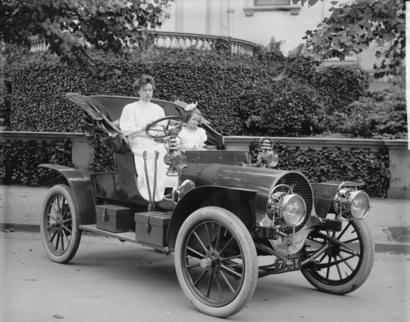
\includegraphics[width=\linewidth]{sample-franklin}
%   \caption{1907 Franklin Model D roadster. Photograph by Harris \&
%     Ewing, Inc. [Public domain], via Wikimedia
%     Commons. (\url{https://goo.gl/VLCRBB}).}
%   \Description{A woman and a girl in white dresses sit in an open car.}
% \end{figure}

% Your figures should contain a caption which describes the figure to
% the reader.

% Figure captions are placed {\itshape below} the figure.

% Every figure should also have a figure description unless it is purely
% decorative. These descriptions convey what’s in the image to someone
% who cannot see it. They are also used by search engine crawlers for
% indexing images, and when images cannot be loaded.

% A figure description must be unformatted plain text less than 2000
% characters long (including spaces).  {\bfseries Figure descriptions
%   should not repeat the figure caption – their purpose is to capture
%   important information that is not already provided in the caption or
%   the main text of the paper.} For figures that convey important and
% complex new information, a short text description may not be
% adequate. More complex alternative descriptions can be placed in an
% appendix and referenced in a short figure description. For example,
% provide a data table capturing the information in a bar chart, or a
% structured list representing a graph.  For additional information
% regarding how best to write figure descriptions and why doing this is
% so important, please see
% \url{https://www.acm.org/publications/taps/describing-figures/}.

% \subsection{The ``Teaser Figure''}

% A ``teaser figure'' is an image, or set of images in one figure, that
% are placed after all author and affiliation information, and before
% the body of the article, spanning the page. If you wish to have such a
% figure in your article, place the command immediately before the
% \verb|\maketitle| command:
% \begin{verbatim}
%   \begin{teaserfigure}
%     \includegraphics[width=\textwidth]{sampleteaser}
%     \caption{figure caption}
%     \Description{figure description}
%   \end{teaserfigure}
% \end{verbatim}